\documentclass[bachelor, english]{algothesis}
% possible types: bachelor, master, zula (seminar, practical)
% Für Seminararbeiten und Praktikumsberichte die Vorlage my-seminar-praktikum.tex verwenden!
% possible languages: english, german

\usepackage[utf8]{inputenc}
\usepackage{xtab}
\usepackage[T1]{fontenc}
\usepackage{lmodern}
\usepackage{caption}
\usepackage{algpseudocode}
\captionsetup[figure]{name=Fig.}
\addto\captionsngerman{
    % Second argument is singular, third is plural
    \crefname{figure}{figure}{figure}
    \Crefname{figure}{Figure}{Figure}
}
\graphicspath{{figures/}}

%%%%%%%%%%%%%%%%%%%%%%%%%%%%%%%%%%%%%%%%%%%%%%%%%%%%%%%%%%%%%%%%%%%%%%%%%%
%%%%%%%%%%%%% Bitte nur ab hier Änderungen vornehmen %%%%%%%%%%%%%%%%%%%%%

\title{The Track Layout Problem from a SAT-Solving Perspective} % Geben Sie hier den Titel Ihrer Arbeit an.

\author{Simon Szulik} % Geben Sie Ihren Namen an.

\newcommand{\abgabedatum}{29. February 2024} % Hier wird das Abgabedatum angepasst

\supervisors{% Geben Sie die Namen aller Betreuenden an, getrennt durch das Makro '\and'
Jun.-Prof.\ Dr.\ Philipp Kindermann \and
Prof.\ Dr.\ Stefan Näher}


\begin{document}

\begin{abstract}
	Bachelor- und Masterarbeiten bedürfen einer Zusammenfassung english
\end{abstract}

\begin{germanabstract}
	Bachelor- und Masterarbeiten bedürfen einer Zusammenfassung deutsch
\end{germanabstract}

\thesistableofcontents

%%%%%%%%%%%%%%%%%%%%%%%%%%%%%%%%%%%%%%%%%%%%%%%%%%%%%%%%%%%%%%%%%%%%%%%%%%%%%%%%
\chapter{Introduction}

\section{Background and Motivation}
In the dynamic field of computer science, graph problems are critical in addressing a wide range of complex challenges, from network design to optimization tasks. The Track Layout Problem (TLP) is one of them. TLP focuses on allocating paths efficiently in a network while optimizing space and resources. Despite its practical importance, TLP is an NP-hard problem, so traditional solutions are frequently impractical. This is where the viewpoint of SAT solvers becomes interesting. By converting the problem into a series of logical clauses, SAT solvers provide an efficient and feasible approach to problem solving. The purpose of this study is to investigate the potential and limitations of SAT-based approaches to TLP, with the goal of gaining a better understanding of the problem and its solutions.

\section{Objectives and Structure of the Study}
This thesis delves into the SAT formulations of the Track Layout Problem, aiming to identify the most efficient formulation for its resolution. We employ a SAT interpretation, where the problem is precisely defined using clauses and variables, and the solution is represented as a configuration of these variables. Our primary goal is to minimize the number of clauses, thereby optimizing the solution approach and creating formulas that can be evaluated as fast as possible. This involves comparing different SAT formulations to determine if one markedly outperforms the other. \newline
The study begins with an overview of graphs, visualization, and related layouts, using examples for comparative analysis. It then introduces the realm of SAT solving, dedicating a chapter to formulating the TLP as a SAT formula and encompassing various methods and approaches. The subsequent sections focus on implementing and testing these algorithms, followed by a separate chapter that is dedicated to the test data that will be used for evaluation. This chapter will detail the types of data selected and how they are instrumental in assessing the effectiveness of the different SAT formulations. This will ensure that the study's findings, which are evaluated in the last part of the work, are grounded in robust and relevant data. The final chapter will discuss potential improvements for future research and propose ideas for additional studies to address potential problems discovered during the study.

\chapter{Fundamentals}

\section{Graph Layouts and Visualization}
\begin{definition}
    A \emph{graph} in graph theory comprises a set of \emph{nodes} and the relationships or connections between them, known as \emph{edges}.
\end{definition}
\noindent
Therefore, graphs are a mathematical representation of physical networks like metrosystems, road networks, and telecommunication structures, but they can also represent abstract networks such as social networks, phylogenetic networks and many more. These graphs can be represented in a variety of ways, including adjacency lists, adjacency matrices, incidence matrices and set notations, each of which offers a distinct perspective and utility for a wide range of computational and analytical tasks. This remarkably  abstract sort of graph representation, however, is frequently difficult to grasp. As a result, a visual representation of graphs is often used in addition to the traditional methods.

\begin{definition}
    A \emph{graph layout} is a visual representation of a given graph in which the node and edge positions are chosen to suit particular aesthetic and functional criteria, depending on the specific needs and nature of the graph being visualized.
\end{definition}
\noindent
A graph layout's primary objective is to depict the diagram's structure in a manner that is both clear and straightforward, ensuring that the reader can effortlessly gain insights and interpret the information presented within the graph. This clarity in presentation is paramount for effective communication. Another significant advantage is that graphs, when visually portrayed, often encapsulate and convey a wealth of information, surpassing what text-only representations can offer. Moreover, the graphical representation of graphs serves as a powerful tool for the swift identification of patterns, clusters, or anomalies in data. \newline
Venturing into the more abstract realm of theoretical computer science, the importance of visualization becomes even more pronounced. This is especially true when delving into the intricacies of understanding and dissecting graph-based algorithms. By employing a graph's graphical representation, researchers and students can acquire a visual insight into the various phases and operations of an algorithm. Such a visual approach not only demystifies the underlying logic and structure of the algorithm but also provides a platform for an intuitive evaluation of its efficiency and overall performance. In the process, visualization can serve as a sentinel, highlighting potential errors or inconsistencies lurking within an algorithm. It's worth noting that a meticulously crafted graphical representation can often expedite and sharpen the comprehension of intricate algorithms and their subsequent impact on a graph, far more than a text-based or formal narrative might \cite{Visualization}. \newline
Before we dive into some instances of graph layouts and visualizations, let's go over some general considerations for graph layout quality and optimization. There are obviously several techniques and algorithms for constructing graph layouts, and the best one is frequently decided by the type of graph and the unique use case. The optimality of a graph layout is also dependent on the scenario, and depending on this, different qualities are used. In the following, we will look more closely at a few interesting aesthetic variables that influence the overall experience with different graph visualization \cite{aesthetic}. The first two properties are the most important to our task, and are extremely important in the comparable yet distinct layouts we will examine next.

\begin{itemize}
    \item \textbf{Clear Visibility of Nodes and Edges (Orthogonality)}: All nodes and edges should be clearly visible and distinguishable from one another, allowing viewers to quickly identify individual parts as well as understand the graph's interactions and connections without misunderstanding or ambiguity. This could for example be done by fixing the nodes and edges to an orthogonal grid.
    \item \textbf{Minimising Edge Crossings}: Edge crossings in a graph should be avoided since they can diminish legibility greatly, leading to confusion and possibly misinterpretation of the shown data. A well-organized graph promotes clarity by reducing these crossings, allowing the reader to easily detect relationships and connections within the graph. Additionally, reducing edge crossings aids in the maintenance of a clean and organized visual structure, which is especially important in complicated networks with many nodes and connections. This method not only improves the graph's overall aesthetic appeal, but also assures that the information it represents is correct and easy to understand.
    \item \textbf{Maximum Angles}: Maximizing the smallest angle between edges in graph drawings improves readership by eliminating clutter and overlap, resulting in clearer node connections and routes. This method simplifies tracing paths and comprehending the structure of the graph by naturally revealing its hierarchical or relational data. Furthermore, it facilitates in distinguishing between distinct graph pieces, making complex information more accessible and easier to evaluate.
    \item \textbf{Symmetry}: Improving symmetry in graph designs increases not only readability and aesthetic appeal, but also allows for faster recognition of patterns and relationships. Symmetric patterns make it easier to compare different areas of the graph, resulting in a more effective conveyance of information and insights. Furthermore, this symmetry can assist in emphasizing major data points and patterns, making the graph more intuitive and user-friendly for analysis and interpretation.
    \item \textbf{Edge Bending}: A graph with too many edge bends can lose clarity, resulting in a cluttered look that obscures node connections and the overall structure of the network. This complexity can impede quick grasp of relationships and patterns, as well as contribute to data misinterpretation, particularly in large networks where good visual representation is critical for effective analysis.
\end{itemize}

\subsection{Stack Number Layout}
\begin{definition}
    The \emph{stack number layout} (also called \emph{book embedding}) represents a graph in which the nodes are arranged along a common line called the \emph{spine} of the book. The edges of the graph are then distributed over \emph{pages} of the book. A page corresponds to a half-plane bounded by the spine.
\end{definition}
\noindent
A graph's book thickness $b$ (also known as page number, stack number, and fixed outerthickness) is defined as the least number of half-planes for any book embedding of the graph. Ollmann's 1973 definition \cite{book_thickness} of graph book thickness is an important measure in graph theory, concentrating on the optimization of graph layouts within a limited space. This idea is especially important in domains like computational geometry and network analysis, where visual clarity and effective space usage are critical. \newline
By minimizing edge overlap, the book embedding method not only improves the legibility of the graph but also plays an important role in algorithmic graph theory. It provides a formal framework for examining graph features and difficulties, particularly in thick graphs where edge crossings can make comprehension difficult. Because of its success in decreasing visual complexity, this method is a valuable tool for both theoretical study and practical data visualization applications.

\subsection{Queue Number Layout}
\begin{definition}
    In the \emph{queue number layout}, the graph's vertices are restricted to a line, while the edges are represented by distinct half-planes above and below this line, referred to as \emph{queues}.
\end{definition}
\noindent
The aim in this representation, first defined by Heath and Rosenberg in 1992 \cite{queue_layout}, to obtaining a linear arrangement of nodes along a baseline and assigning the graph's edges to queues in a way that precludes nesting of independent links inside the same queue. This approach attempts to organize the graph's structure in a clear, sequential manner, with the queue number $q$ representing the least number of queues required for every possible queue configuration of the graph. Unlike the stack number, which is ordered last-in-first-out, the queue structure is ordered first-in-first-out, providing a unique perspective in graph representation. This strategy is particularly successful at emphasizing the graph's directed flow of data and interactions, making it easier to follow and analyze. Similar to the stack number layout, one of the key goals of this layout method is to reduce edge crossings, hence considerably improving the overall readability and interpretability of the graph.

\subsection{The Track Layout Problem}
    \label{chap:track}
\begin{definition}
    A \emph{graph track layout} is a division of its vertices into sequences called \emph{tracks}, with the vertices in each sequence forming an independent set and the edges between each two pairs of tracks forming a non-crossing set.
\end{definition}
\noindent
We are now dealing with the track layout problem, which is a well-known subject in graph drawing and consequently the true topic of this study, in which we exclusively inspect undirected graphs. The track layout, like queue and stack number layouts, is an arrangement of graphs with the same purposes, including clarity and readability. Dujmovi et al. were the first to define this problem \cite{track_layout}. The TLP, also referred to as the k-track problem, is concerned with determining the fewest number of tracks called track-number $t$ for which the nodes of the graph can be distributed among them, according to the following rules:
\begin{enumerate}
    \item \textbf{Uniqueness}: Each node is on precisely one track.
    This rule works in the same way as the previously discussed aesthetic of visibility.
    \item \textbf{Adjacent Nodes}: Adjacent nodes of the graph must not be on the same track, which prevents edges from running within a track.
    \item \textbf{No Crossings}: This implies that there are no edges $(u,w)$ and $(i,j)$ for which $u$ comes before $i$ in one track, but $w$ comes after $j$ in another track. It is important to note that this regulation prohibits only the act of crossing if the start- and endnodes of the edges are on the same track. To better understand this rule some examples of forbidden crossings as well as an example of an allowed edge crossing is depicted in \cref{fig:crossings} below.
\end{enumerate}

\begin{figure}[ht]
    \centering

    \begin{subfigure}[b]{0.45\linewidth}
        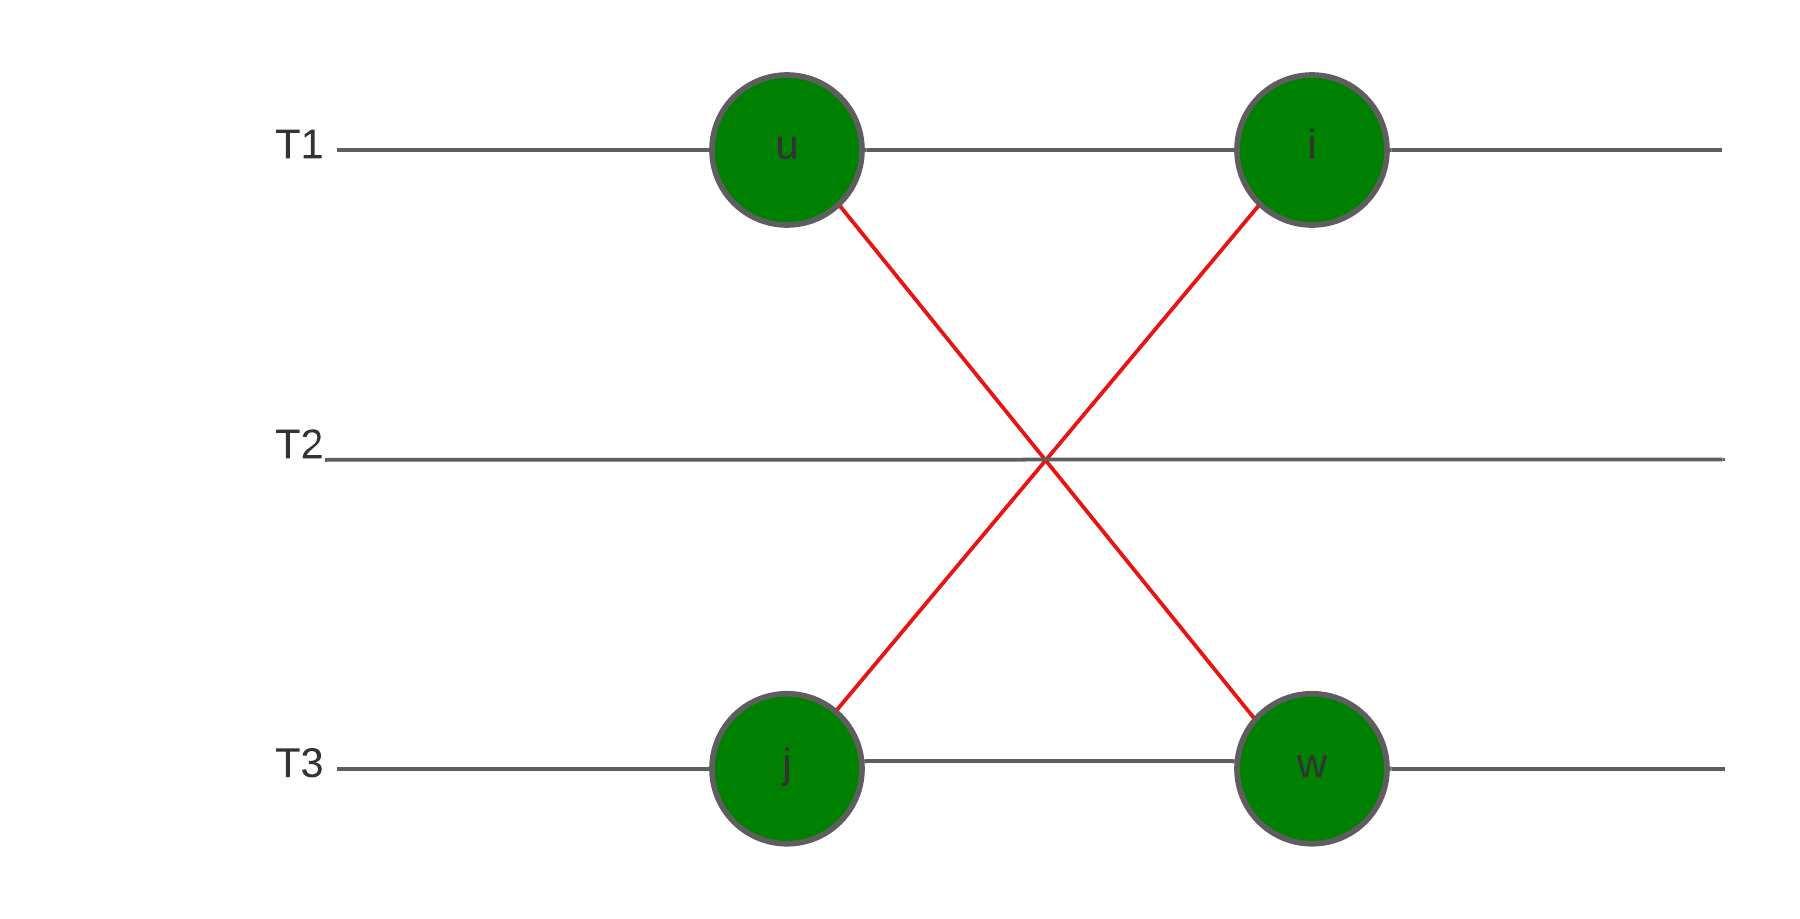
\includegraphics[width=\linewidth]{figures/Verbot2.png}
        \caption{Forbidden Crossing through more Tracks}
        \label{fig:verbot2}
    \end{subfigure}
    \hfill
    \begin{subfigure}[b]{0.45\linewidth}
        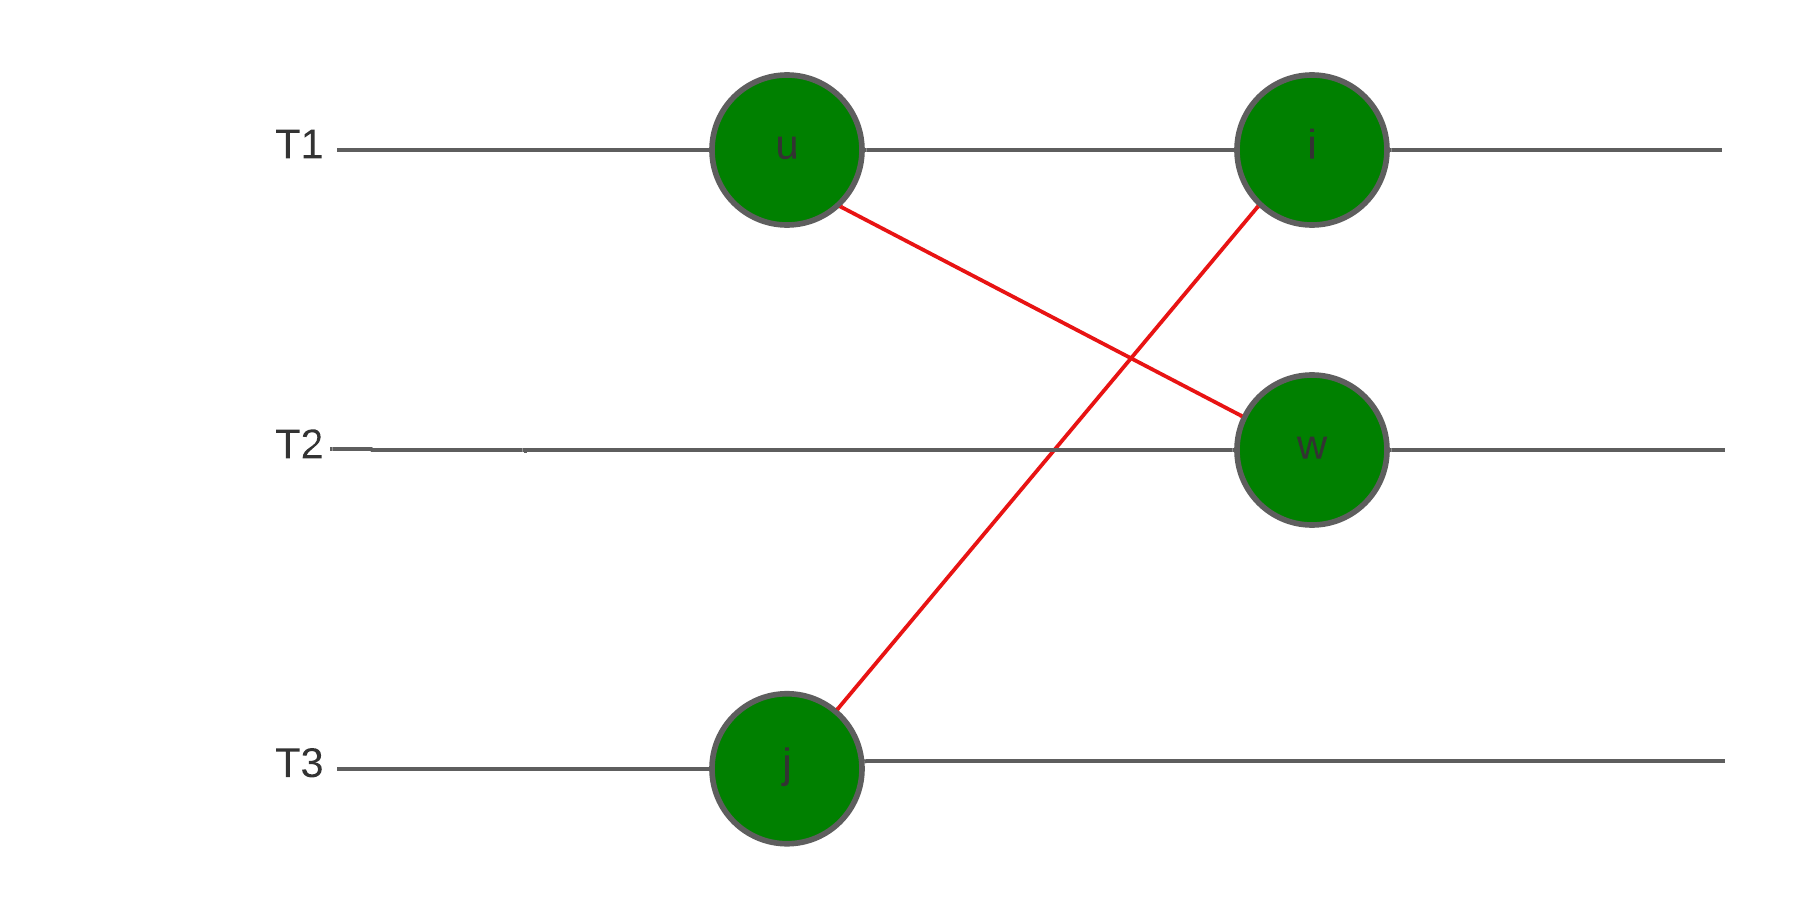
\includegraphics[width=\linewidth]{figures/Erlaubt.png}
        \caption{Allowed Crossing}
        \label{fig:erlaubt}
    \end{subfigure}

    \begin{subfigure}[b]{0.9\linewidth}
        \centering
        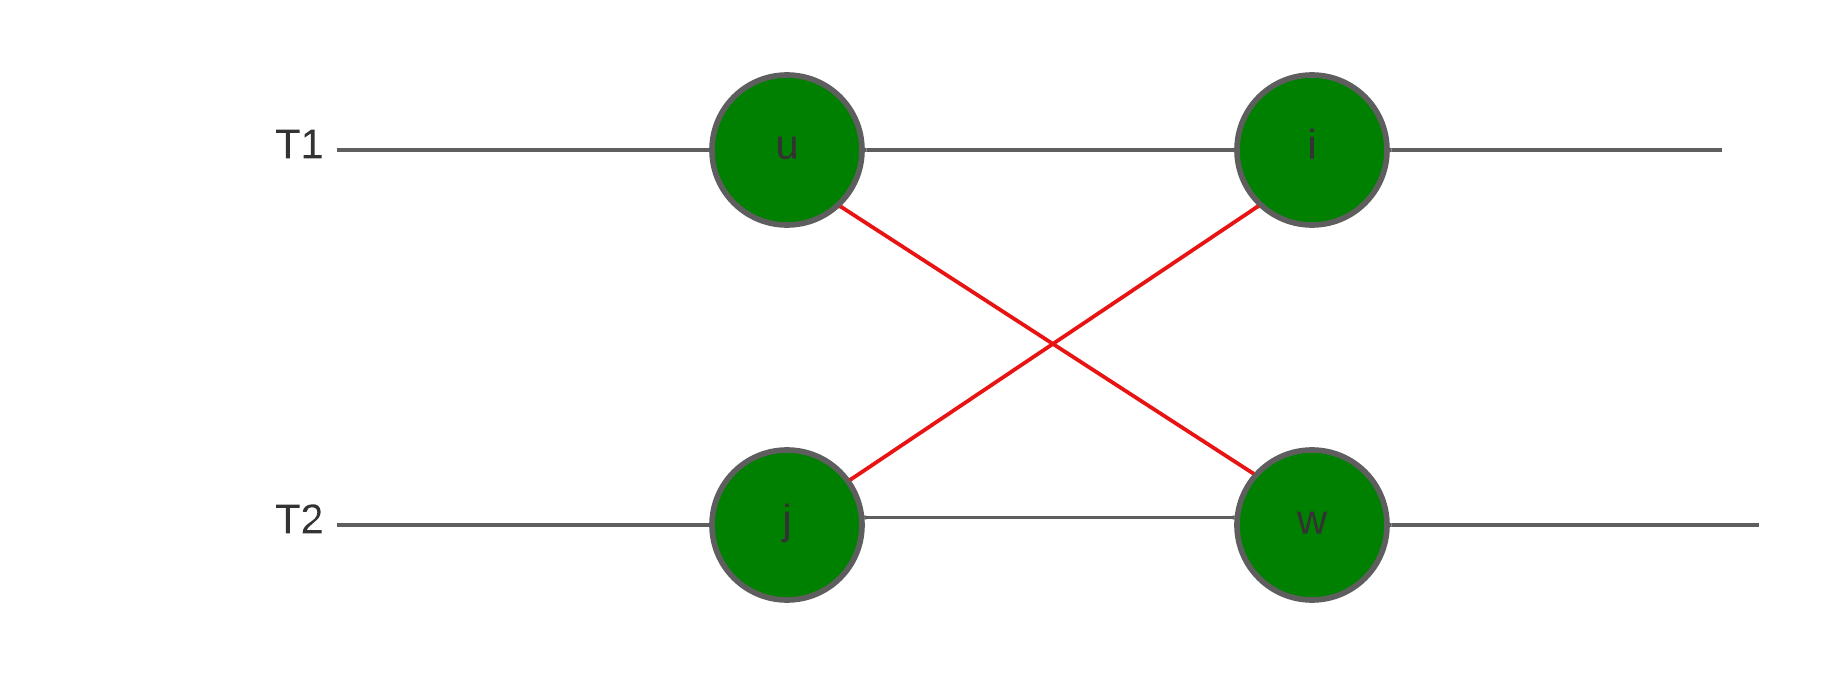
\includegraphics[width=0.7\linewidth]{figures/Verbot1.png}
        \caption{Forbidden Crossing in Adjacent Tracks}
        \label{fig:verbot1}
    \end{subfigure}

    \caption{Forbidden and Allowed Crossings}
    \label{fig:crossings}
\end{figure}
\clearpage

\subsection{Example}
The following illustrations serve to differentiate and visualize the differences between the three layouts and helps us to be able to discern between them. \Cref{fig:octahedron} shows an octahedron, a polyhedron with eight faces, twelve edges, and six vertices, with four edges meeting at each vertex. Below this, you can see \cref{fig:octahedron_graph}, that shows a graph represetation in which each vertex is connected to the surrounding vertices that span the triangular surfaces of the object.

\begin{figure}[ht]
    \centering
    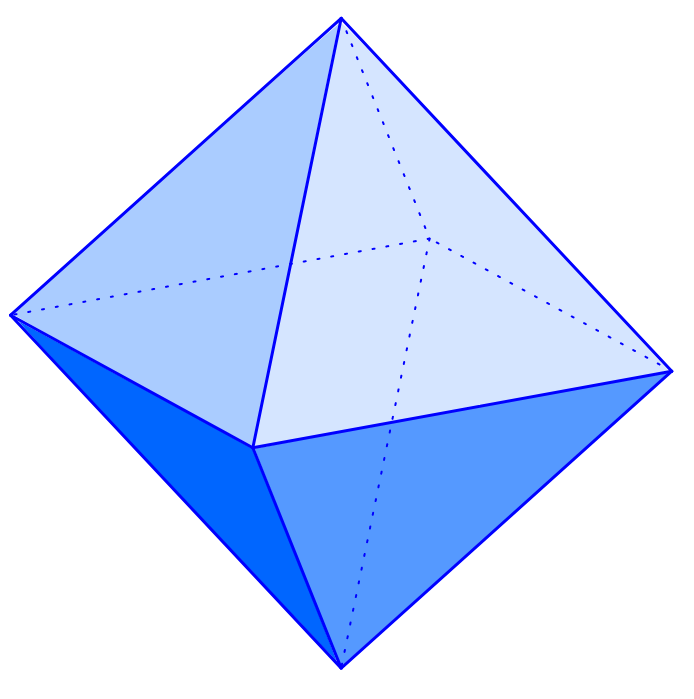
\includegraphics[width=0.5\linewidth]{figures/octahedron.png}
    \caption{Octahedron \protect\footnotemark}
    \label{fig:octahedron}
\end{figure}

\begin{figure}[ht]
    \centering
    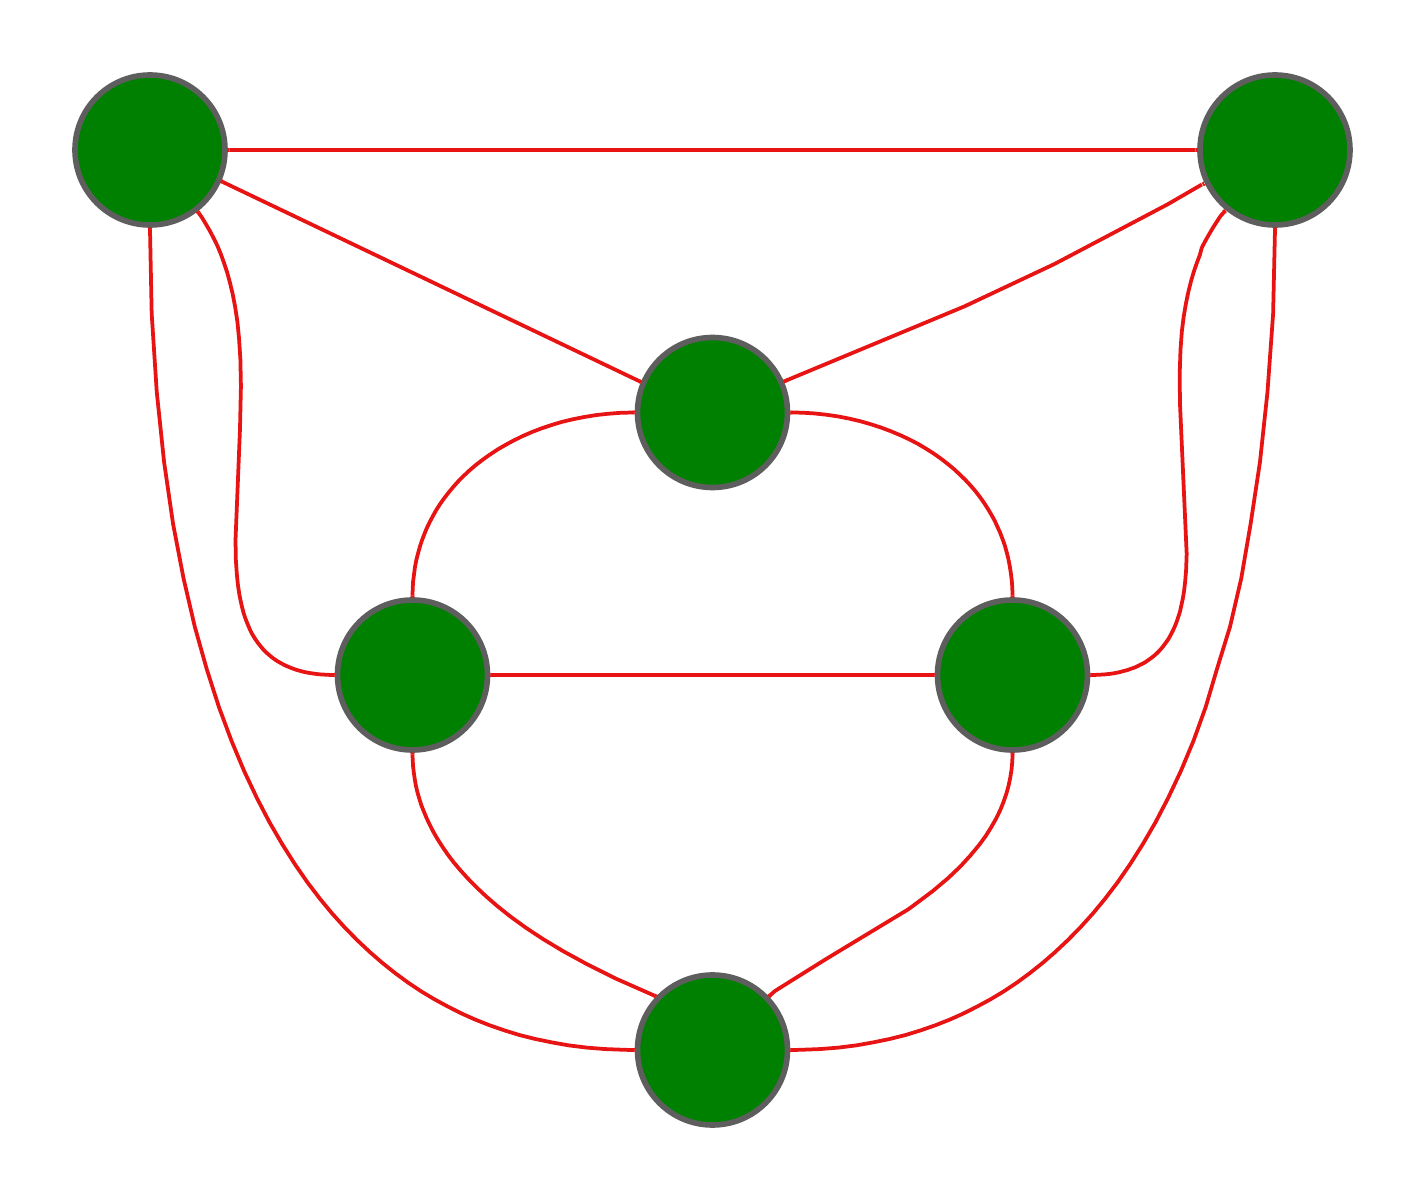
\includegraphics[width=0.525\textwidth]{figures/octahedron_graph.png}
    \caption{Graph Interpretation of an Octahedron}
    \label{fig:octahedron_graph}
\end{figure}
\footnotetext{Rosemark, \textit{octahedron}, cleanpng.com, 30.11.2023}
\noindent
This graph can now be shown as a book embedding, in the form of a queue layout as well as using the track layout. The three visualisations shown in \cref{fig:octahedron_layouts} clearly highlight the differences between the layouts. While the book embedding divides the graph into distinct pages or layers to ensure non-crossing edges, the queue number layout organizes the edges into queues, aiming for a compact representation. It is noticeable that three tracks are required to represent the graph as a track layout. The other two alternatives just necessitate the use of two stacks respectively queues to display the same graph.

\begin{figure}[ht]
    \centering

    \begin{subfigure}[b]{0.45\linewidth}
        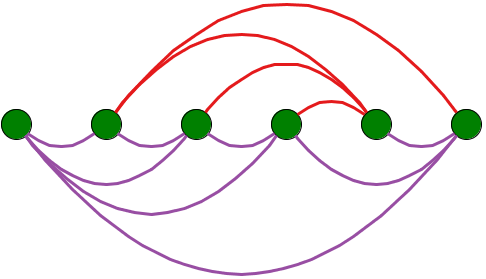
\includegraphics[width=\linewidth]{figures/octahedron_stack.png}
        \caption{Octahedron Graph drawn in 2 Stacks}
        \label{fig:octahedron_stack}
    \end{subfigure}
    \hfill
    \begin{subfigure}[b]{0.45\linewidth}
        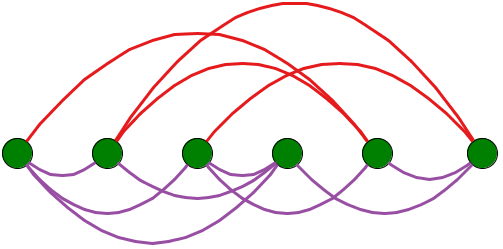
\includegraphics[width=\linewidth]{figures/octahedron_queue.png}
        \caption{Octahedron Graph drawn in 2 Queues}
        \label{fig:octahedron_queue}
    \end{subfigure}

    \begin{subfigure}[b]{0.45\linewidth}
        \centering
        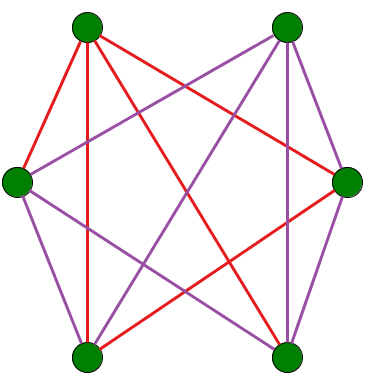
\includegraphics[width=0.8\linewidth]{figures/octahedron_tlp.png}
        \caption{Octahedron Graph drawn in 3 Tracks}
        \label{fig:octahedron_tlp}
    \end{subfigure}

    \caption{Octahedron Graph drawn in different Layouts \protect\footnotemark}
    \label{fig:octahedron_layouts}
\end{figure}

\footnotetext{Sergey Pupyrev, \textit{octo}, spupyrev.github.io/linearlayouts.html, 30.11.2023}

\clearpage

\section{Introduction to SAT-Solving}
Propositional logic has long been regarded as a foundation of reasoning in philosophy and mathematics. Its formalization as Boolean algebra was accompanied by the discovery, that a large range of combinatorial problems can be represented as propositional satisfiability (SAT) problems. As a result, SAT solving became an important method in theoretical computer science and mathematical logic. It needs to solve SAT problems, which question whether it is possible to provide truth values to a Boolean formula in order for it to evaluate to true. This topic is not simply of academic interest, but it also has significant practical relevance because it underpins various applications in cryptography, software verification, artificial intelligence, and optimization problems. Understanding the structure of those logical issues is critical to understanding the difficulty and utility of SAT solving. \newline
Conjunctive Normal Form (CNF) is commonly used to write SAT problems, in which a formula is an AND relation of many phrases and each clause is an OR relation of literals. A literal in this sense is a Boolean variable or its negation. Despite the fact that the structure's simplicity hides the potential complexity of the difficulties, its elegance allows for a consistent approach to problem solving. SAT solvers, sophisticated algorithms that use advanced methods like backtracking, unit propagation, and clause learning to answer these issues, aid in the resolution of these problems. The evolution of these solvers throughout time is a monument to the inventiveness and perseverance of field researchers. Initially impossible issues are now frequently tackled, illustrating the extraordinary efficacy of these techniques. However, the difficulties in SAT solving exist, particularly when dealing with extremely large or convoluted issues. \newline
The topic of SAT solving research is dynamic and continuing, driven by the constant attempt to improve the efficiency of algorithms and heuristics. This search is not only intellectual; the ramifications in our world of complicated decision-making are far-reaching. Advances in SAT solving carry the potential of uncovering answers to some of the most difficult and convoluted issues in computer science and beyond \cite{Sat_solving}.

\subsection{Complexity}
Within the field of computational computability, problem complexity is an essential aspect. Specifically, the classification of issues into several complexity classes and levels of difficulty. The study of NP-hard issues is a key component and a large area of research attention. These issues are well-known for being computationally challenging and are crucial to comprehending algorithms and their bounds.

\begin{definition}
    An \emph{NP-hard problem} refers to being at least as difficult as the most difficult problem in the NP complexity class. Any NP-hard problem in polynomial time can be reduced to any NP-hard problem in polynomial time. This means that if one NP-hard problem can be solved effectively (in polynomial time), then so can all NP problems.
\end{definition}
\noindent
The satisfiability problem of propositional logic also belongs to this class of problems. Furthermore, it has been proven to be NP-complete. Nevertheless, NP-hard problems are not necessarily in NP, i.e., they are not guaranteed to be verified in polynomial time. Because of its NP-hardness, the SAT serves as the foundation for classifying additional problems as NP-hard. If a problem can be reduced to SAT in polynomial time, it is also considered NP-hard \cite{SAT_Complexity}. When we look at the TLP through the lens of SAT, we get a boolean formula whose satisfiability determines whether there is a layout that follows the rules. This consideration will be important in our further experiments. If it is not immediately evident whether there are configurations that satisfy the formula or clauses that signal unfulfillability, all conceivable configurations must be checked in order to reach a solution. This could result in much longer processing times for larger variable sets.

\section{Related Work}
Looking at mathematical problems and general computer science problems from a sat perspective is ubiquitous. Although graph problems are uncommon, they can still be solved using a propositional interpretation. In their paper "The Book Embedding Problem from a SAT-Solving Perspective," bekos et al. examined one of these graph problems \cite{book_embedding_sat}. The researchers presented a simple and straightforward SAT formulation for graph queue number layout. They attempted to solve some non-trivial instances of this problem set in a reasonable amount of time using their SAT-formulation. Furthermore, various hypotheses about planar graphs were tested, and a lower bound of 4 for $b$ for 1-planar graphs was discovered. The following work is based on the methods and formulations shown by bekos et al. and deals with the TLP in a similar way.

\chapter{SAT Formulations for the TLP}
Let $G = (V,E)$ be the graph we consider in our problem, where $V =\{v_1,v_2,...,v_n\}$ represents the vertices, and $E = \{e_1,e_2,...,e_n\}$ the corresponding edges of the graph. The primary objective is to determine whether there exists a Tracklayout $L$ for this graph that meets the conditions outlined in the previous section. To tackle this challenge, we first frame the problem in terms of a logical formula, denoted as $F(G, t)$. This formula seeks to address the problem by encoding it into a SAT instance. It's important to highlight that the formula is deemed satisfied if and only if there exists a layout $L$ that displays the initial graph $G$ on $t$ tracks. Our formula will hold the conjunctive normal form (CNF). The formula $F(G, t)$ is defined by its set of variables and the associated set of rules. The primary role of these rules is to ensure the correct assignment of the variables. They are expressed in a specific type of propositional logic, which can be  transformed into CNF clauses straightforwardly \cite{conjunction}. In the following sections, we will define the variables we will need for our SAT formulation and examine various clause approaches that will help us comply with the ruleset.

\section{Variables \& Clauses}
\label{sec:vars_clauses}
\subsection{Basic Variables and Clauses}
\label{sec:basic_clauses}
%Wie viele klauseln gibt es jeweils zu transitivität und assymetrie und dem andren ? \\

The variables of $F(G, t)$ model a track layout of $G$ on $t$ tracks, if such a structure exists. To assign a node of the graph to a track, we use the variable $\sigma(v_i,t_k)$ for each pair of node $v_i \in V$ and track t. For instance, the assignment $\sigma(v_1, t_1)$ is considered true when node $v_1$ is positioned on track $t_1 \,$ in $\, L$. In order to formulate all possible assignments for each node on every track, a total of $ \vert V \vert \times t$ variables are required. We may now assign a track to each node using this variable. In order to fulfill the first rule of the TLP, the uniqueness, we must verify that each node is on at most one track, which requires our first clauses. To maintain clarity, we will approach this in two parts, whereby the first one guarantees that every node is on at least one track:
    $$ (\sigma(v_i,t_1) \lor \sigma(v_i,t_2) \lor \dots \lor \sigma(v_i,t_n)) \, \forall v_i \in V \text{ and every track }t $$
Therefore, the first part of each of the clauses will contain $t$ variables. Next, we have to confirm that every node is on at most one track, which combined with the first part will ensure that for each node precisely one of the track variables $\sigma$ evaluates to true, i.e. that each node is assigned to exactly one track. The second part is formulated as follows:
    $$ (\overline{\sigma(v_i, t_x) \land \sigma(v_i, t_y)}) \, \forall v_i \in V \text{ and every combination of two tracks } x, y \text{ with } x \neq y$$
\noindent
As outlined, we will ignore the diagonal of the track-combinations. Also note that due to commutativity $(\lnot \sigma(v_i, t_x) \lor \lnot \sigma(v_i, t_y))$ is the same as $(\lnot \sigma(v_i, t_y) \lor \lnot \sigma(v_i, t_x))$. This assumptions helps us to reduce the number of variables by a significant amount and thus obtain a total number of $\frac{(\vert V \vert^2-\vert V \vert)}{2}$ disjunctions of two negated literals each resulting in $2 \times \frac{(\vert V \vert^2-\vert V \vert)}{2}$ variables for the second part of this rule. All in all, when we merge these two parts, we need $\vert V \vert$ larger clauses with $t + 2 \times \frac{(\vert V \vert^2-\vert V \vert)}{2}$ variables each to establish the first rule. The next clauses enforce that neighboring nodes are on the same track and require us to include the edges of the graph in our formulation. This can be achieved by adding the following conjunctions:
        $$ \forall e_{i,j} \in E : (\overline{\sigma(v_i,t_x) \land \sigma(v_j,t_x)}) \text{ for every track } t $$
This phrasing leads to a total of $\vert E \vert \times t$ clauses with one negated conjunction each, or more precisely $2 \times (\vert E \vert \times t)$ variables per clause. With the help of the clauses defined so far, we can now assign a unique track to each node without breaking the rules of the TLP.

\subsection{First Approach on Crossing Edges}
Now we turn our attention to the core problem of the track layout, namely the restriction of forbidden crossings. To detect crossings in the layout, we first need a way to determine the position of the nodes within the tracks. The simplest way to arrange the nodes would be to include a variable that assigns each node a unique number that indicates its position along the tracks. Therefore, we define the tuple $\phi(v_i,p)$ for each $v_i \in V$ and $p$ up to the total number of nodes. Hence $\phi(v_i,p)$ is true, when $v_i$ is on position $p$. Note that the nodes are taken in a total order, so we can assume that for each node $v$ exactly one variable $\phi(v_i,p)$ must be true. Ultimately this method results in ${\vert V \vert}^2$ variables to express all possible orders. Furthermore, clauses would be required to ensure that no two nodes are in the same position. This specification works equivalent to rule 1 and results in $\vert V \vert$ clauses with $\vert V \vert + 2 \times \frac{(\vert V \vert^2-\vert V \vert)}{2}$ variables. To better understand this definition, let's take a look at the \cref{fig:order_example_tot} below.

\begin{figure}[ht]
  \centering
  \begin{minipage}{0.6\textwidth}
    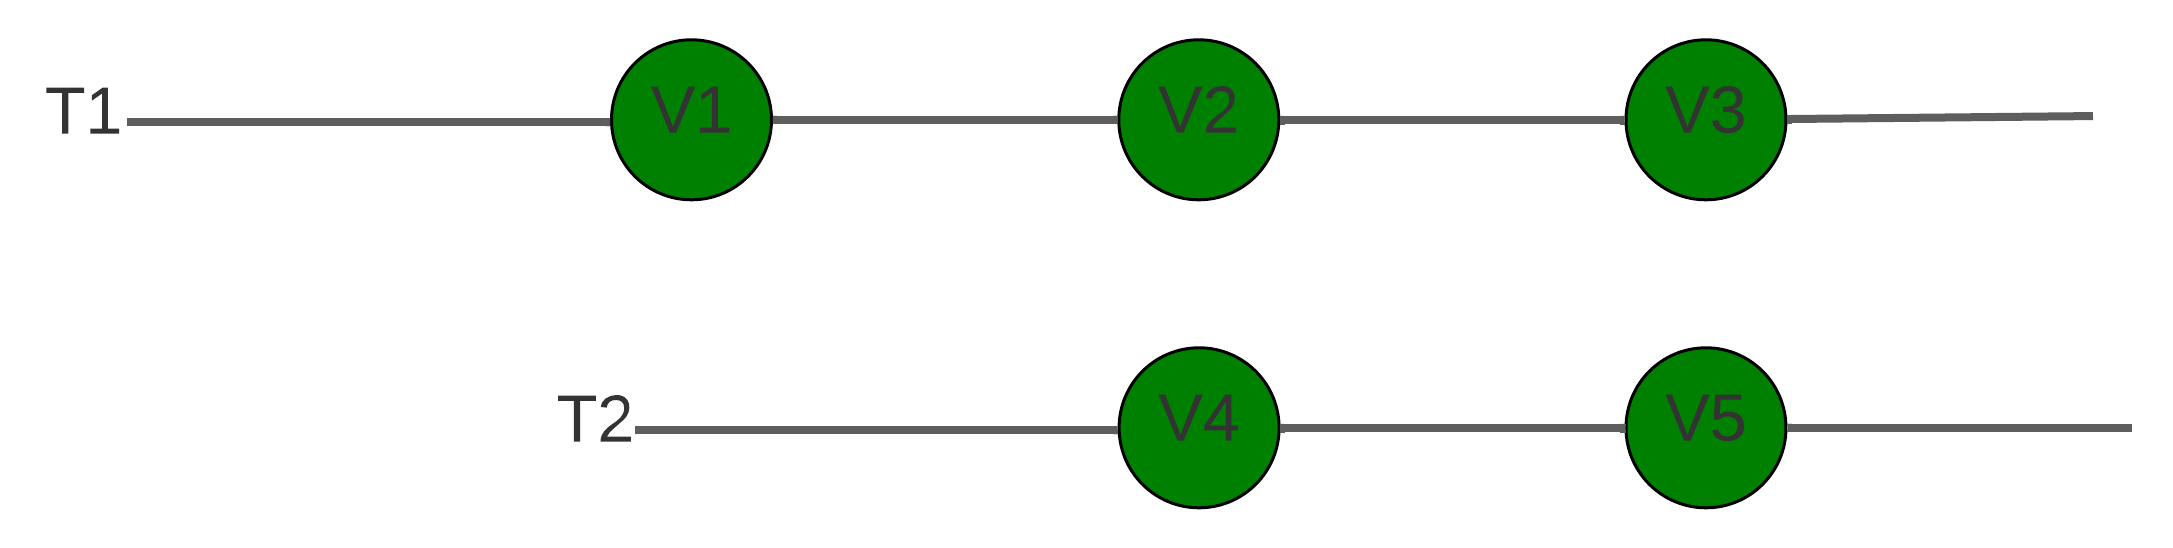
\includegraphics[width=\linewidth]{figures/Order_example.png}
  \caption{Example for Total Ordering}
  \label{fig:order_example_tot}
  \end{minipage}%
  \begin{minipage}{0.4\textwidth}
    To formulate this sequence of nodes, these variables must come true:
    \begin{itemize}
    \item  $\phi(v_1,1)$, $\phi(v_2,2)$, $\phi(v_3,3)$, $\phi(v_4,4)$ and $\phi(v_5,5)$
    \end{itemize}
  \end{minipage}
\end{figure}
\noindent
It is critical to remember that $\phi$ alone is insufficient to define a distinct sequence, as it does not provide any information about the tracks on which the nodes are distributed. To correctly formalize the preceding example, the following five variables must also be set to true:
$$\sigma(v_1, t_1), \sigma(v_2, t_1), \sigma(v_3, t_1), \sigma(v_4, t_2) \text{ and } \sigma(v_5, t_2)$$
\noindent
Next, we must exclude all possibilities of forbidden crossings. To accomplish this, we create the following formula using $\phi$ and $\sigma$:
    $$ \forall e_{i,j}, e_{u,w} \in E, \ \forall m,n,a,b \text{ in range of } \vert V \vert \text{ with } m<n, \, a<b:$$
    $$(\overline{\sigma(v_i,t_x) \land \sigma(v_u,t_x) \land \sigma(v_j,t_y) \land \sigma(v_w,t_y) \land \phi(v_i,p_m) \land \phi(v_u,p_n) \land}$$
    $$ \overline{\phi(v_w,p_a) \land \phi(v_j,p_b)})\text{ for all disjoint pair of tracks } t_x \text{ and } t_y $$
To have a better understanding of this rather larger formula, we shall analyze it in further detail. Since we are considering edge pairs, we need $\vert E \vert^2$ clauses. Logically, we do not consider self-edges or in other words non-disjoint edge pairs and get a total of $(\vert E \vert^2 - \vert E \vert)$ as our first factor. In addition, there will be another one for the disjoint track pairs. As  commutativity also works in our favor here we only have to care about one of the pairs $(t_x, t_y)$ and $(t_y, t_x)$. The corresponding alternative can already be covered while calculating the clauses for the first one. Adding $\frac{(t^2-t)}{2}$ clauses for the tracks, the only thing missing is the inclusion of the appropriate positions. We first choose two positions for $m$ and $n$. Let these be distinct, but fixed. Since we operate on a total order, each position may only occur once. Therefore we know that the number of remaining positions for $a$ and $b$ must be two less. Summarised for this interpretation we gain a total of
$ (\vert E \vert^2 - \vert E \vert)) \times \frac{(t^2-t)}{2} \times \frac{(\vert V \vert^2-\vert V \vert)}{2} \times \frac{((\vert V \vert-2)^2-(\vert V \vert-2))}{2}$ clauses.
\noindent \newline
At first glance, the problem seems to have been solved. However, the positioning of the nodes among the individual tracks seems to cause a problem, as we have not yet introduced any restrictions for the track transitions. The distribution within a track also poses a similar kind of problem with this formulation. The first approach appears to be missing conditions to create a unique variable assignment. Looking at the example in \cref{fig:order_example_tot}, $\phi$ appears to be a valid method of storing the vertexes order. On the other hand, just designating the position variables does not guarantee that the nodes in $T$ are consecutively numbered. In our illustration, $\phi(v_2,2)$ and $\phi(v_3,3)$ are set to true, but $\phi$ itself is not fixed according to the current definition and would therefore have to be interpreted individually for each pair of nodes. For this reason, it has not yet been assured that node $v_2$ is located to the left of node $v_3$.
The same applies to all other node pairs for each track. In order to maintain a clear position of the nodes in relation to each other, we need to introduce rules to prevent certain configurations. \newline
One way to define the exact position in $L$ would be to force a node $v_i$ with $\sigma(v_i,t_1)$ to the first position with the help of further clauses, and to force another node $v_j$ with $\sigma(v_j,t_{max})$ to the last position. This should be repeated until you have a correct setup by setting nodes to the second and second last positions, third and third last positions, etc. Another alternative would be to look at the relationship between nodes. To do this, for each node $v_i$ and $\sigma(v_i, t_y)$, state that all other nodes $v_j$ with $\sigma(v_j, t_x)$ and $t_x < t_y$ have a position that is smaller than than the position of $v_i$ and have a greater position than $v_i$ if $t_x > t_y$. However, this ideas appears to require an excessive amount of effort and would increase the number of clauses considerably for the fact that it only limits the problematic areas we have using this method. As the approach of structuring the nodes on the basis of a single total order does not seem suitable, we will not consider it further for the time being.
\subsection{Second Approach on Crossing Edges}
\label{sec:approach2}
To more precisely specify the order, we require variables that allow us to view and compare the neighboring nodes for each node in L. We can also prohibit crossings if we have access to all nodes and their neighbors on the respective tracks. As a result, we are now taking a different approach and defining a new variable $\omega$ to determine the relationship between two nodes. We define this variant as the tuple $\omega(v_i,v_j)$ for each $v_i,v_j \in V$. This variable evaluates to true if $v_i$ is one of the left neighbors of $v_j$ on any track.  Notice that variables $\omega(v_i,v_j)$ with $i = j$ can not evaluate as true, because this will be referred to $v_i$ and $v_j$ being the same node, that can obviously can not be the left neighbor of itself. This will eventually lead to ${\vert V \vert}^2$ variables. In this relative encoding of the sequence between nodes, clearly asymmetry has to hold for these variables, which will be ensured by the following rule:
    $$ \omega(v_i,v_j) \leftrightarrow \lnot \omega(v_j,v_i) $$
To reduce the total set of clauses by a substantial sum, we define the asymmetry of the variable $\omega(v_i,v_j)$ only for the case that $i < j$. The other literals $\omega(v_i,v_j)$ with $i > j$ can replaced with the respective counterpart $\lnot \omega(v_j,v_i)$ leading to $\frac{(\vert V \vert^2-\vert V \vert)}{2}$ clauses \cite{asymmetric}. In order to establish a proper order within a track, we must also ensure transitivity with in total ${\vert V \vert}^3$ clauses. This is done as follows:
    $$ \omega(v_i,v_j) \land \omega(v_j,v_k) \rightarrow \omega(v_i,v_k) \, \forall \text{ pairwise distinct } v_i,v_j,v_k \in V$$
Additionally, we implement $t \times {\vert V \vert}^2$ clauses which cause that a node can only lie to the left of another node if both nodes are
positioned on the same track. If this requirement did not exist, there would be considerable difficulties with the track breaks of the eventual node positioning:
    $$ \omega(v_i,v_j) \rightarrow \sigma(v_i,t_k) \land \sigma(v_j,t_k) \, \forall \text{ pairwise distinct } v_i,v_j \in V \text{and every track }t$$
Therefore, it is important to note that there are indeed nodes $v_i$ for which none of the variables $\omega$ with $\omega(v_i,v_n) \forall v_n \in V$ evaluates to true. This is precisely the case when the node n is on the right edge of the track. We will again point  this method out with help of the same example in \cref{fig:order_example_rel} we looked at before to truly understand the definition of this order implementation.

\begin{figure}[ht]
  \centering
  \begin{minipage}{0.6\textwidth}
    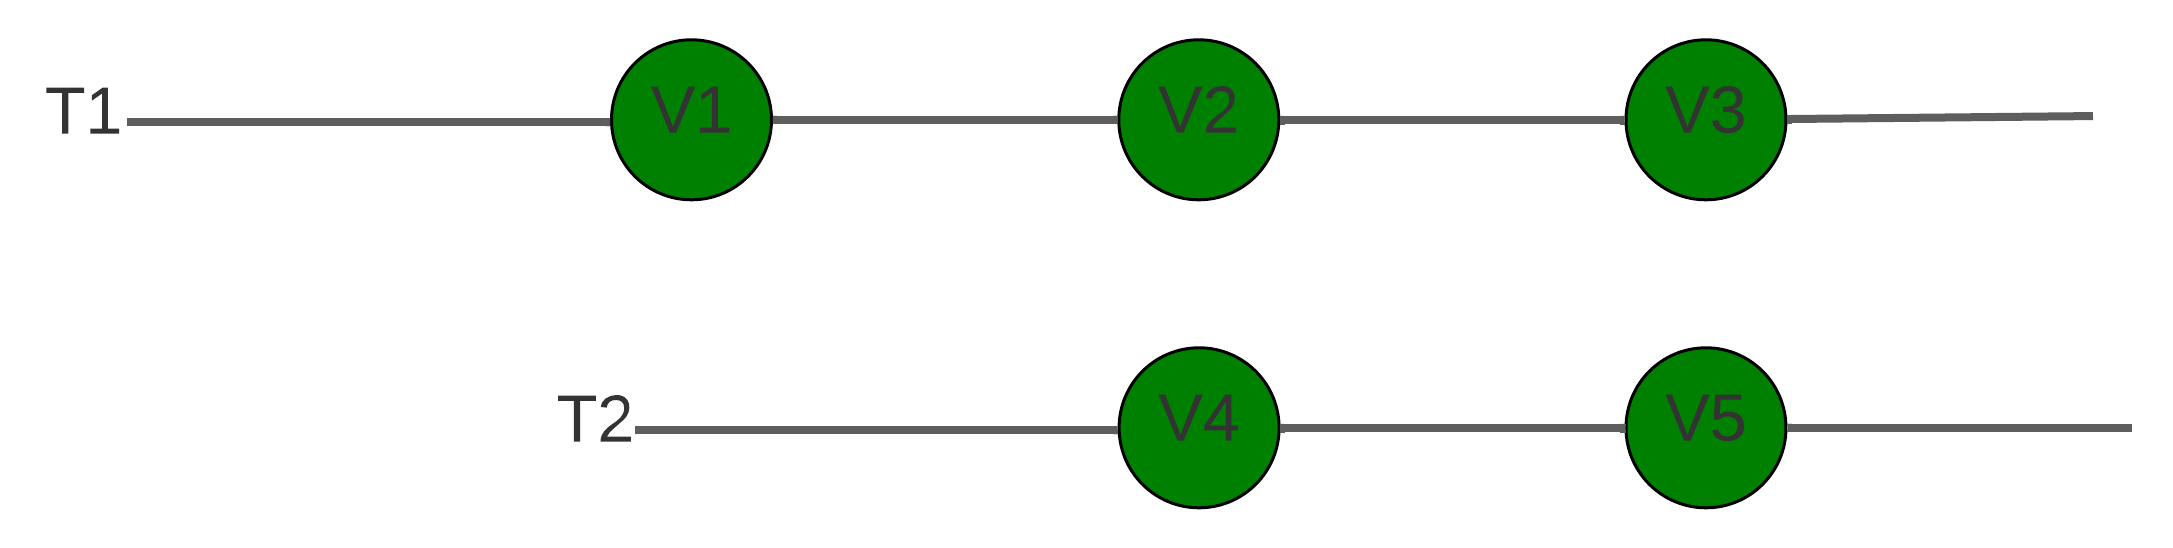
\includegraphics[width=\linewidth]{figures/Order_example.png}
  \caption{Example for Relational Ordering}
  \label{fig:order_example_rel}
  \end{minipage}%
  \begin{minipage}{0.4\textwidth}
    To formulate this sequence with the relational method, these variables must come true:
    \begin{itemize}
    \item  $\omega(v_1,v_2)$, $\omega(v_1,v_3)$, $\omega(v_2,v_3)$ and $\omega(v_4,v_5)$
    \end{itemize}
  \end{minipage}
\end{figure}
\noindent
Remember that $\omega$ alone is not enough to provide the complete track layout. Next, we have to block the intersections of edges using our new approach. This can be reached with the following conjunctions which we build for each disjoint pair of edges $e_{i,j}, e_{u,w}$ so that:
    $$ \forall e_{i,j}, e_{u,w} \in E : \overline{(\sigma(v_i,t_x) \land \sigma(v_u,t_x) \land (\sigma(v_j,t_y) \land (\sigma(v_w,t_y) \land}$$
    $$ \overline{\omega(v_i,v_u) \land \omega(v_w,v_j)}\text{ for all disjoint pair of tracks } t_x \text{ and } t_y $$
Using this method, we can cut out a whole factor that was used to define the positions in the total order. We don't need to manifest the position of the nodes in an own variable, since we can also extract an unique order from only the relations between each node. At the end, this results in
$ (\vert E \vert^2 - \vert E \vert)) \times \frac{(t^2-t)}{2}$ clauses with 6 negated variables each.

\subsection{Third Approach on Crossing Edges}
\label{sec:approach2_2}
In general, there are numerous ways to improve SAT formulas. In our third attempt, we reduced the number of clauses as well as their size. We use the same foundation as in the second approach. Looking at the previous formula, it is interesting to note that we used an entire loop to handle the track pairs. The next consideration is what possibilities there are to reduce this factor. \newline
One idea for looking beyond this loop is to define a new variable that indicates that two nodes are on the same track. According to this formula, it doesn't matter which track the nodes are on, as long as they're on the same one. We therefore define a new variable $\psi$ for which $\psi(v_i,v_j) \forall v_i,v_j \in V$ evaluates to true if and only if $v_i$ and $v_j$ are on the same track. With the introduction of a new variable, we are obviously increasing the general handling of our phrases while needing ${\vert V \vert}^2$ variables for every possibility of every two nodes being on the same track. To apply this variable correctly, we need additional clauses that enforce our interpretation of $\psi$. Similar to the implication for the correctness of $\omega$ formulated in the second approach, we need $t \times {\vert V \vert}^2$ clauses which are worded as follows:
    $$ \sigma(v_i,t_k) \land \sigma(v_j,t_k)\rightarrow \psi(v_i,v_j) \, \forall v_i,v_j \in V \text{and every track }t$$
With the help of this new variable, it is possible to limit the crossing clauses. Again we have to formulate a conjunction which we construct for every disjoint pair of edges $e_{i,j} e_{u,w}$ in order that:
    $$ \forall e_{i,j}, e_{u,w} \in E : \overline{(\psi(v_i,v_u) \land \psi(v_j,v_w) \land   \omega(v_i,v_u) \land \omega(v_w,v_j)}$$
This formulation allows us to ignore another factor in our quantity of clauses and so on decrease the required clauses to $ (\vert E \vert^2 - \vert E \vert))$ and reduce the variables per clause by two. As we rated the first approach as significantly worse and not finished, we will analyze the second and third version for their quality and evaluation speed. For the following comparison, we hypothesise the following
\begin{enumerate}
    \item[H1:] The second version significantly reduces the largest clause in our formula, requiring far less time to create.
    \item[H2:] Despite having more variables, the formula created by the second approach will take much less time to evaluate based on the set size of clauses.
\end{enumerate}


\chapter{Implementation in Python}
Even though Python may not offer the same performance as lower-level programming languages (such as C/C++), we will opt for it to implement the TLP and its solution approaches. Python has certain benefits, like readability and flexibility, which are very helpful for the nested loops that make up the clauses. Furthermore, we have easy access to Sat-Solvers through the variety of libraries, which we can use to create, modify, and solve our formula.

\section{Introduction to the Python-SAT Library}
PySAT is a Python library for editing, solving and analysing Boolean formulas and SAT (Satisfiability) problems. Born out of the need to create a unified and efficient collection of tools for SAT-related tasks in Python, PySAT integrates a number of widely used state-of-the-art SAT solvers such as MiniSat, Glucose and Lingeling. The library allows users to efficiently formulate Boolean formulas and analyse solutions, making it a valuable tool in research and development. Overall, PySAT provides an efficient and flexible platform for working on a wide range of Boolean logic and optimisation problems. Its ease of use and performance make it a popular choice for many scientific and industrial applications. \newline
Among the numerous core modules of the pysat toolkit, we will mainly use formula and solvers. While solvers are Python wrappers for the code originally implemented in the C/C++ languages, the formula module is a pure Python module. Boolean variables in PySAT are represented using natural numbers, with $\mathbb{N}^+\setminus\{0\}$. According to this representation, a literal is an integer, with $-1$ representing the literal $\lnot x_1$ and $5$ representing the literal $x_5$. Moreover a clause refers to a set of literals, with $[-3, -2]$ being an example of a clause $(\lnot x_3 \lor \lnot x_2)$ \cite{PySAT}. Once you have created variables and clauses, you can easily add them to a formula and have it solved by any solver contained in the library. The important thing here is that the formulae that the solver requires for evaluation are always converted into a CNF. The solve() method returns an assignment of the variables if the formula has a solution, or a false if the solution set is empty. \newline
To evaluate the formulas for solving the TLP in the following, we use the SAT solver lingeling. Lingelin is a fork of the PrecoSAT prototype. It's data structures are designed to take up much less space. Large clauses with four or more literals, for example, are stored separately on literal stacks, and the literals of these large clauses with four or more literals are referred to as enced in the occurrence lists not with pointers but through their stack position. Finally, occurrence lists are implemented as integer stacks that live in a single large integer stack called the occurrences stack and are again referenced by stack position. This reduces the size on 64-bit machines from 24 to 8 bytes \cite{LingeLing}.

\section{Implementation of the SAT Formulations}
With the help of PySAT, it is possible to create our desired variables in the form of 2D arrays. The variable $\sigma$, as defined in \hyperlink{alg:sigma}{algorithm 1}, is interpreted in such a way that $\sigma[v_i][t_k]$ is true, when node $v_i$ is on track $t_k$ or else false.

\begin{algorithm}[ht]
    \caption{Implementation of $\sigma$}
    \label{alg:sigma}
        $\, \, \, \sigma = [][]$ \newline
        $name = 0$ \newline
        \For{node in range(nodes)}{
            \For{track in range(tracks)}{
                $ \, \, \, \sigma [\text{node}][\text{track}] = name$ \newline
                $name \; = name + 1$
            }
            \, $\text{formula.append($\sigma$[node][track] for track in range(tracks))}$ \newline
            \For{comb in combination($\sigma$[node][track] for track in range(tracks), 2)}{
                \, $\text{formula.append([-comb[0], -comb[1]])}$
            }
        }
\end{algorithm}
\noindent
Implementing this nested loop, we create all $ \vert V \vert \times t$ variables we need to determine the corresponding track of each node. In addition, we need to verify that $\sigma$ is working properly. The first rule is straight-forward to follow because we don't need to create an extra method for it. Instead, we can directly append the relevant negated conjunctions inside the second loop while initializing $\sigma$. Lines 4 and 5, both inside the outer for, ensure that each node must be on exactly one track. The variables $\omega$ and $\psi$ are realised equivalently using the steps depicted in line 1 to 3, whereby the inner loop is adjusted according to the quantity of variables ($ \vert V \vert \times \vert V \vert$) mentioned in chapter \ref{sec:vars_clauses}. $\omega[v_i][v_j]$ will be evaluated as true, if $v_i$ is a left neighbor of $v_j$ on any track $t$. Each variable $\psi[v_i][v_j]$ will be referred to as true if, and only if $v_i$ and $v_j$ are on the same track $t$. To implement the clauses regarding the the second rule, a for-loop is needed that iterates through a list of all edges and adds the clauses that prevent the two nodes from lying on the same track. By keeping in mind that we have to add this clauses for every track we end up with \hyperlink{alg:second_rule}{algorithm 2}.

\begin{algorithm}[ht]
    \caption{Implementation of the 2. TLP Rule}
    \label{alg:second_rule}
        \For{edge in Edges}{
            \For{track in range(tracks)}{
                $\text{formula.append(-$\sigma$[edge[0]][track], -$\sigma$[edge[1]][track])}$
            }
        }
\end{algorithm}
\noindent
In order to implement our second approach and thus the final variant of the position variable, we need to create clauses that preserve the correctness of the formulation. The asymmetry observed in \hyperlink{alg:assymetric}{algorithm 3} is simple to achieve. For the transitivity seen in \hyperlink{alg:transitivity}{algorithm 4} it is important to remember that the rule requires three in pairs disjoint nodes. Therefor we need to add another if condition that was was left out in this notation due to readability. To introduce the last rule regarding $\omega$ we again need some nested loops. Adding the clause shown in \hyperlink{alg:edgeCase}{algorithm 5} to our formula, prevents $\omega[v_i][v_j]$ from evaluating as true if $v_i$ and $v_j$ are not on the same track.
\begin{algorithm}[ht]
    \caption{Asymmetry of $\omega$}
    \label{alg:assymetric}
        \For{leftNode in range(nodes)}{
            \For{rightNode in range(nodes)}{
                \If{leftNode < rightNode}{
                    \For{track in range(tracks)}{
                        $\text{formula.append(-$\sigma$[leftNode][track], -$\sigma$[rightNode][track],}$
                        $\text{\, \, \, \, \, \, \, \, \, \, \, \, \, \, $\omega$[leftNode][rightNode], $\omega$[rightNode][leftNode])}$
                    }
                    $\text{formula.append(-$\omega$[leftNode][rightNode], -$\omega$[rightNode][leftNode])}$
                }
            }
        }
\end{algorithm}

\begin{algorithm}[ht]
    \caption{Transitivity of $\omega$}
    \label{alg:transitivity}
        \For{leftNode in range(nodes)}{
            \For{middleNode in range(nodes)}{
                \For{rightNode in range(nodes)}{
                   $\text{formula.append(-$\omega$[leftNode][middleNode], -$\omega$[middleNode][rightNode],}$
                   $\text{\, \, \, \, \, \, \, \, \, \, \, \, \, \, \,$\omega$[leftNode][rightNode])}$

                }
            }
        }
\end{algorithm}

\begin{algorithm}[ht]
    \caption{Edge Case and Track Breaks including $\omega$}
    \label{alg:edgeCase}
        \For{leftNode in range(nodes)}{
            \For{rightNode in range(nodes)}{
                \For{track in range(tracks)}{
                    \If{leftNode != rightNode}{
                        $\text{formula.append(-$\omega$[leftNode][rightNode], -$\sigma$[leftNode][track],}$
                        $\text{\, \, \, \, \, \, \, \, \, \, \, \, \, \, \,$\sigma$[rightNode][track])}$
                    }
                }
            }
        }
\end{algorithm}
\noindent
This leaves the implementation of the restriction of edge crossings and the corresponding clauses to determine the correct order of the nodes. Since we do not need any major additions to set up the two viable approaches and the corresponding clauses in sections \ref{sec:approach2} and \ref{sec:approach2_2} are already in a form that is favorable for us, we will not look at the algorithms for this in more detail. The quantity of nests, nevertheless, is what makes the unique techniques intriguing. To illustrate why the first approach is not considered further, let's take a look at the basic implementation of the individual methods. Derived from the formula for the restriction clauses, we obtain two very small loops which only include the edge pairs and the track pairs. The remaining information we need to prohibit crossings in these implementations is retrieved from the well defined variables $\omega$ and $\psi$. These variants and its difference can be viewed in algorithm \hyperlink{alg:edgeRestriction2.1}{6} and \hyperlink{alg:edgeRestriction2.2}{7}.
\begin{algorithm}[ht]
    \caption{Implementation of Edge Restriction with $\omega$}
    \label{alg:edgeRestriction2.1}
        \For{edgePair in range(edgePairs)}{
            \For{trackPair in range(trackPairs)}{
                $\text{formula.append(...)}$
            }
        }
\end{algorithm}

\begin{algorithm}[ht]
    \caption{Implementation of Edge Restriction with $\omega$ and $\psi$}
    \label{alg:edgeRestriction2.2}
        \For{edgePair in range(edgePairs)}{
            $\text{formula.append(...)}$
        }
\end{algorithm}
\noindent
The first approach can be seen in \hyperlink{alg:edgeRestriction1}{algorithm 8}. It is easy to recognise the large number of interconnected loops, which is one of the biggest problems of this approach. This depth of nesting means that the generation of the clauses alone takes a considerable amount of time for larger graphs.
\begin{algorithm}[ht]
    \caption{Implementation of Edge Restriction with $\phi$}
    \label{alg:edgeRestriction1}
        \For{edgePair in range(edgePairs)}{
            \For{trackPair in range(trackPairs)}{
                \For{a in range(nodes)}{
                    \For{b in range(nodes)}{
                        \For{c in range(nodes)}{
                            \For{d in range(nodes)}{
                                $\text{formula.append(...)}$
                            }
                        }
                    }
                }
            }
        }
\end{algorithm}

\section{Test Cases and Results}
\subsection{Dataset}
Since the utilization of robust and diverse datasets is a crucial point for the advancement of algorithmic researches, we decided to get our Data from a well known Graph Layout Benchmark Datasets \cite{Benchmark}. The accessed source contains a list of benchmark datasets for testing graph layout algorithms, whereby the collection was originally summarized and is maintained by the Northeastern University Visualization Lab. Therefore we decided to use the \textbf{Rome-Lib} Dataset that was collected by Di Battista et al\text{.} and first introduced in their paper  \glqq An experimental comparison of four graph drawing algorithms\grqq \, in 1995 \cite{Rome_Lib}. Using this dataset that provides a wide array of diverse graphs all within a range of $10$ to $100$ nodes, we choose $100$ undirected graphs in total to evaluate our algorithms. In order to cover the widest possible variety of cases and graph sizes, the set of test graphs contained $10$ graphs with $10\times n$ nodes each. More preciesly, 10 graphs with 10 nodes each, 10 graphs with 20 nodes each, etc. The individual test graphs and their rough properties are listed in % hier noch ref zu tabellen
\\

\begin{minipage}{0.5\textwidth}
\tablefirsthead{\hline Name & Nodes & Edges \\ \hline}
\begin{xtabular}{|c|c|c|}
% Ihre Daten für die erste Tabelle
grafo1972.10.gml & 10 & 15.0 \\
grafo1098.10.gml & 10 & 9.0 \\
grafo327.10.gml & 10 & 10.0 \\
grafo898.10.gml & 10 & 9.0 \\
grafo210.10.gml & 10 & 10.0 \\
grafo460.10.gml & 10 & 9.0 \\
grafo949.10.gml & 10 & 10.0 \\
grafo1627.10.gml & 10 & 15.0 \\
grafo2538.10.gml & 10 & 10.0 \\
grafo254.10.gml & 10 & 11.0 \\
\hline
grafo270.20.gml & 20 & 30.0 \\
grafo3051.20.gml & 20 & 23.0 \\
grafo413.20.gml & 20 & 24.0 \\
grafo1024.20.gml & 20 & 21.0 \\
grafo2922.20.gml & 20 & 24.0 \\
grafo1837.20.gml & 20 & 24.0 \\
grafo1716.20.gml & 20 & 23.0 \\
grafo2396.20.gml & 20 & 24.0 \\
grafo1901.20.gml & 20 & 26.0 \\
grafo874.20.gml & 20 & 25.0 \\
\hline
grafo176.30.gml & 30 & 35.0 \\
grafo358.30.gml & 30 & 39.0 \\
grafo1246.30.gml & 30 & 36.0 \\
grafo1334.30.gml & 30 & 39.0 \\
grafo484.30.gml & 30 & 35.0 \\
grafo1627.30.gml & 30 & 40.0 \\
\end{xtabular}
\end{minipage}%
\begin{minipage}{0.5\textwidth}
\tablefirsthead{\hline Name & Nodes & Edges \\ \hline}

\begin{xtabular}{|c|c|c|}
% Ihre Daten für die zweite Tabelle
grafo4620.60.gml & 60 & 75.0 \\
grafo9484.60.gml & 60 & 78.0 \\
grafo6483.60.gml & 60 & 83.0 \\
grafo1192.60.gml & 60 & 79.0 \\
grafo5896.60.gml & 60 & 84.0 \\
grafo8586.60.gml & 60 & 79.0 \\
grafo4436.60.gml & 60 & 78.0 \\
grafo7448.60.gml & 60 & 81.0 \\
grafo5483.60.gml & 60 & 75.0 \\
grafo4376.60.gml & 60 & 73.0 \\
\hline
grafo1381.70.gml & 70 & 87.0 \\
grafo9300.70.gml & 70 & 96.0 \\
grafo8237.70.gml & 70 & 98.0 \\
grafo7992.70.gml & 70 & 94.0 \\
grafo9739.70.gml & 70 & 85.0 \\
grafo8105.70.gml & 70 & 100.0 \\
grafo8187.70.gml & 70 & 89.0 \\
grafo4558.70.gml & 70 & 92.0 \\
grafo9297.70.gml & 70 & 96.0 \\
grafo9569.70.gml & 70 & 91.0 \\
\hline
grafo9582.80.gml & 80 & 101.0 \\
grafo5370.80.gml & 80 & 111.0 \\
grafo4865.80.gml & 80 & 117.0 \\
grafo9096.80.gml & 80 & 108.0 \\
grafo9797.80.gml & 80 & 107.0 \\
grafo4890.80.gml & 80 & 108.0 \\
\end{xtabular}
\end{minipage}

\clearpage

\begin{minipage}{0.5\textwidth}
\tablefirsthead{}
\begin{xtabular}{|c|c|c|}
% Ihre Daten für die erste Tabelle
grafo1687.30.gml & 30 & 32.0 \\
grafo1623.30.gml & 30 & 41.0 \\
grafo4040.30.gml & 30 & 36.0 \\
grafo1958.30.gml & 30 & 33.0 \\
\hline
grafo7330.40.gml & 40 & 50.0 \\
grafo7000.40.gml & 40 & 50.0 \\
grafo10615.40.gml & 40 & 50.0 \\
grafo7121.40.gml & 40 & 50.0 \\
grafo5675.40.gml & 40 & 44.0 \\
grafo10402.40.gml & 40 & 47.0 \\
grafo3335.40.gml & 40 & 53.0 \\
grafo6115.40.gml & 40 & 46.0 \\
grafo9997.40.gml & 40 & 50.0 \\
grafo5772.40.gml & 40 & 49.0 \\
\hline
grafo3744.50.gml & 50 & 72.0 \\
grafo4603.50.gml & 50 & 69.0 \\
grafo6775.50.gml & 50 & 63.0 \\
grafo6838.50.gml & 50 & 60.0 \\
grafo4945.50.gml & 50 & 69.0 \\
grafo1528.50.gml & 50 & 56.0 \\
grafo3780.50.gml & 50 & 63.0 \\
grafo3685.50.gml & 50 & 72.0 \\
grafo6740.50.gml & 50 & 66.0 \\
grafo6264.50.gml & 50 & 72.0 \\
\hline
\end{xtabular}
\end{minipage}%
\begin{minipage}{0.5\textwidth}
\tablefirsthead{}

\begin{xtabular}{|c|c|c|}
% Ihre Daten für die zweite Tabelle
grafo9795.80.gml & 80 & 117.0 \\
grafo7907.80.gml & 80 & 127.0 \\
grafo8058.80.gml & 80 & 111.0 \\
grafo5558.80.gml & 80 & 108.0 \\
\hline
grafo8959.90.gml & 90 & 121.0 \\
grafo8840.90.gml & 90 & 117.0 \\
grafo8494.90.gml & 90 & 119.0 \\
grafo7130.90.gml & 90 & 125.0 \\
grafo8558.90.gml & 90 & 125.0 \\
grafo8952.90.gml & 90 & 128.0 \\
grafo8756.90.gml & 90 & 117.0 \\
grafo8946.90.gml & 90 & 125.0 \\
grafo8711.90.gml & 90 & 121.0 \\
grafo3756.90.gml & 90 & 127.0 \\
\hline
grafo8793.100.gml & 100 & 138.0 \\
grafo10633.100.gml & 100 & 138.0 \\
grafo10820.100.gml & 100 & 141.0 \\
grafo10750.100.gml & 100 & 135.0 \\
grafo8674.100.gml & 100 & 135.0 \\
grafo10153.100.gml & 100 & 136.0 \\
grafo10644.100.gml & 100 & 145.0 \\
grafo10603.100.gml & 100 & 136.0 \\
grafo10998.100.gml & 100 & 142.0 \\
grafo10257.100.gml & 100 & 124.0 \\
\hline
\end{xtabular}
\end{minipage}

\subsection{Specifications}
The various tests were carried out using a machine with the characteristics shown in \cref{tab:specs}.

\begin{table}[h]
\centering
\begin{tabular}{|l|l|}
\hline
\textbf{Component}      & \textbf{Specification}                \\ \hline
Processor       & Intel i5-8250U @ 3.400GHz      \\ \hline
Memory          & 8 GB LPDDR4X RAM               \\ \hline
Storage         & 512 GB SSD                     \\ \hline
Operating System & Linux Mint 21.1 x86\_64        \\ \hline
\end{tabular}
\caption{Specifications of Acer Swift 5}
\label{tab:specs}
\end{table}


\chapter{Comparison and Analysis of SAT Formulations}

\section{Efficiency of Different Formulations}

\section{Advantages and Disadvantages of Each Formulation}

\section{Recommendations for Specific Use Cases}


\chapter{Discussion}

\section{Comparison with Existing Solutions and Studies}

\section{Limitations and Possible Extensions}

\section{Outlook on Future Research}


\chapter{Conclusion}

\section{Summary of Key Findings}

%%%%%%%%%%%%%%%%%%%%%%%%%%%%%%%%%%%%%%%%%%%%%%%%%%%%%%%%%%%%%%%%%%%%%%%%%%%%%%%%
\clearpage
\bibliographystyle{mybabalpha-fl}
\bibliography{mybib}


\end{document}
